\documentclass[10pt]{beamer}
\usepackage[utf8]{inputenc} % pour le format de sortie
\usepackage{geometry}
\usepackage[T1]{fontenc}
\usepackage[english]{babel} % pour les accents
\usepackage{csquotes}
\usepackage{enumitem}
\usepackage{amssymb,amsmath,amsthm, amsfonts} % math libraries (amsthm : unumbered theorems)
\usepackage{mathtools} % for psmallmatrix
\usepackage{fancyhdr,multicol,accents, bbm,subcaption,caption,float,verbatim}
\usepackage[all]{xy} % for diagrams with arrows
\usepackage{tikz-cd} % for diagrams with arrows
\usepackage{graphicx} % to manage images
\usepackage{titlesec}
\usepackage{hyperref} % for hyperlinks to refs or bibliography
\usepackage{indentfirst} % for indenting the first line of a paragraph
\usepackage{lmodern}
\usepackage[backend=bibtex]{biblatex} % for bibliography
\usepackage{bookmark}
\usepackage{multimedia}
\addbibresource{refs.bib}

% \usepackage[utf8]{inputenc} % pour le format de sortie
\usepackage[a4paper]{geometry}
\usepackage[T1]{fontenc}
\usepackage[english]{babel} % pour les accents
\usepackage{csquotes}
\usepackage{enumitem}
\usepackage{amssymb,amsmath,amsthm, amsfonts}
\usepackage{mathtools}
\usepackage{fancyhdr,multicol,accents, bbm,subcaption,caption,float,verbatim}
\usepackage[all]{xy} % for diagrams with arrows
\usepackage{tikz-cd} % for diagrams with arrows
\usepackage{graphicx} % to manage images
\usepackage{titlesec}
\usepackage{hyperref} % for hyperlinks to refs or bibliography
\usepackage{indentfirst} % for indenting the first line of a paragraph
\usepackage{optidef}
\usepackage[backend=bibtex, style=alphabetic]{biblatex} % for bibliography
\usepackage{bookmark}
\usepackage{algorithm}
\usepackage{algpseudocode}
\usepackage{chronosys}
\usepackage{csvsimple}
\usepackage{longtable}
\usepackage{caption}
\usepackage{setspace}
\addbibresource{refs.bib}

% Margins, font size =====================================================================================================================
%\oddsidemargin = 0.5cm \evensidemargin = 0.5cm \textwidth = 6.3in
%\oddsidemargin = 1.2cm \evensidemargin = 1.2cm \textwidth = 6.3in
%\textheight =8.6in
\geometry{
	a4paper,
	total={170mm,257mm},
	left=20mm,
	top=20mm,
}

% Sections (theorems, propositions, lemmas…) =====================================================================================================================
\newtheorem{theorem}{Theorem}[section]
\newtheorem{lemma}[theorem]{Lemma}
\newtheorem{corollary}[theorem]{Corollary}
\newtheorem*{conjecture}{\bf Conjecture}
\newtheorem{proposition}[theorem]{Proposition}
% \numberwithin{theorem}{section} % To display the section number in the theorem

\theoremstyle{definition}
\newtheorem{definition}[theorem]{Definition}
\newtheorem{assumption}[theorem]{Assumption}
\newtheorem{exercise}{Exercise}
\newtheorem*{solution}{Solution}
\newtheorem*{answer}{Answer}
\newtheorem*{claim}{Claim}

\theoremstyle{remark}
\newtheorem*{theoremno}{{\bf Theorem}}
\newtheorem*{remark}{Remark}
\newtheorem*{example}{Example}
\newtheorem*{hint}{Hint}



% Commands =====================================================================================================================
\def\bb#1{\mathbb{#1}}
\def\cal#1{\mathcal{#1}}
\def\frak#1{\mathfrak{#1}}
\def\rm#1{\mathrm{#1}}
\def\bf#1{\mathbf{#1}}
\newcommand{\C}{\mathbb{C}}
\newcommand{\R}{\mathbb{R}}
\newcommand{\N}{\mathbb{N}}
\newcommand{\Z}{\mathbb{Z}}
\newcommand{\Q}{\mathbb{Q}}
\newcommand{\K}{\mathbb{K}}
\newcommand{\bbP}{\mathbb{P}}
\newcommand{\F}{\mathcal{F}}
\newcommand{\calP}{\mathcal{P}}
\newcommand{\G}{\mathcal{G}}
\newcommand{\calL}{\mathcal{L}}
\newcommand{\calC}{\mathcal{C}}
\newcommand{\calN}{\mathcal{N}}
\newcommand{\calF}{\mathcal{F}}
\newcommand{\calE}{\mathcal{E}}
\newcommand{\frakA}{\mathfrak{A}}
\newcommand{\frakS}{\mathfrak{S}}
\newcommand{\esp}{\mathbb{E}}
% \P = caracs spéciaux,\S = paragraphe, \L = L barre

% Existe déjà : ker, partie Im, Re, min, max, inf, sup, log, exp, sin, sinh, cos, cosh,, tan lim, liminf, limsup
\DeclareMathOperator{\Id}{Id}
\DeclareMathOperator{\Hom}{Hom}
\DeclareMathOperator{\Ima}{Im}
\DeclareMathOperator{\Homeo}{Homeo}
\DeclareMathOperator{\Aut}{Aut}
\DeclareMathOperator{\Bij}{Bij}
\DeclareMathOperator{\Isom}{Isom}
\DeclareMathOperator{\GL}{GL}
\DeclareMathOperator{\End}{End}
\DeclareMathOperator{\rang}{rang}
\DeclareMathOperator{\rank}{rank}
\DeclareMathOperator{\vol}{vol}
\DeclareMathOperator{\sgn}{sgn}
\DeclareMathOperator{\var}{Var}
\DeclareMathOperator{\erf}{erf}
\DeclareMathOperator{\spec}{spec}
\DeclareMathOperator{\diag}{diag}
\DeclareMathOperator{\pgcd}{pgcd}
\DeclareMathOperator{\pgdc}{pgdc}

% Lois de probabilités
\DeclareMathOperator{\Geom}{Geom}
\DeclareMathOperator{\Bin}{Bin}
\DeclareMathOperator{\Exp}{Exp}
\DeclareMathOperator{\Ber}{Ber}
\DeclareMathOperator{\Student}{Student}
\DeclareMathOperator{\Poi}{Poi}
\newcommand{\czero}{\calC^0}
\newcommand{\cone}{\calC^1}
\newcommand{\ctwo}{\calC^2}
\newcommand{\cinf}{\calC^{\infty}}
\newcommand{\bigpeter}[1]{\Big\langle#1\Big\rangle}
\newcommand{\peter}[1]{\langle#1\rangle}
\newcommand{\transp}[1]{#1^t}
\newcommand{\series}[2]{\sum_{#1}^{\infty}#2}
\newcommand{\intt}[4]{\int_{#1}^{#2}#3\mathrm{d}#4}
\newcommand{\ddt}[1]{\frac{\mathrm{d}#1}{\mathrm{dt}}}
\newcommand{\deldt}[1]{\frac{\partial#1}{\partial\mathrm{t}}}
\newcommand{\rmd}[1]{\mathrm{d}#1}
\newcommand{\inv}[1]{#1^{-1}}
\newcommand{\dx}{\rmd x}
\newcommand{\dy}{\rmd y}
\newcommand{\dz}{\rmd z}
\newcommand{\dt}{\rmd t}
\newcommand{\du}{\rmd u}
\newcommand{\dv}{\rmd v}
\newcommand{\ds}{\rmd s}
\newcommand{\dxy}{\rmd xy}
\newcommand{\dyz}{\rmd yz}
\newcommand{\dyx}{\rmd yx}
\newcommand{\dzy}{\rmd zy}
\newcommand{\dzx}{\rmd zx}
\newcommand{\dxz}{\rmd xz}
\newcommand{\gtinf}[1]{\underset{#1\to\infty}{\longrightarrow}}
\newcommand{\sm}[4]{\begin{psmallmatrix}#1&#2\\#3&#4\end{psmallmatrix}}
\newcommand{\map}[4]{
	\begin{matrix}
		#1&\to&#2\\#3&\mapsto&#4
	\end{matrix}
}


\title[RRLB NMPC]{Study of Relaxed Recentered Log-Barrier function based Nonlinear Model Predictive Control}
\subtitle{(RRLB NMPC)}
\author{Tudor Oancea}
\date{May 2022}
\logo{
\includegraphics[height=1cm]{Logo.pdf}}

\usetheme{Boadilla}
\usecolortheme{beaver}

\def\bb#1{\mathbb{#1}}
\def\cal#1{\mathcal{#1}}
\def\bf#1{\mathbf{#1}}
\def\rm#1{\mathrm{#1}}


\begin{document}

\frame{\titlepage}

\begin{frame}
    \frametitle{Problem formulation - Regular NMPC}
    \begin{align*}
        V_N(x)=\underset{\mathbf{x},\mathbf{u}}{\min} &\quad \sum_{k=0}^{N-1}l(x_k,u_k)~+~F(x_N)\\
        \text{s.t.} &\quad x_0=x\text{ and }x_{k+1}=f(x_k,u_k)\\
        &\quad x_k\in\cal{X}\\
        &\quad u_k\in\cal{U}
    \end{align*}
    with $l(x,u)=x^TQx+u^TRu$ and $F(x)=x^TPx$ ($P$ determined later).
     $\mathcal{X}=\left\{x~|~C_xx\leq d_x \right\}$ and $\mathcal{U}=\left\{u~|~C_uu\leq d_u \right\}$\,.
\end{frame}

\begin{frame}
    \frametitle{Problem formulation - RRLB NMPC}
    \begin{align*}
        \tilde{V}_N(x)=\underset{\mathbf{x},\mathbf{u}}{\min} &\quad \sum_{k=0}^{N-1}\tilde{l}(x_k,u_k)~+~\tilde{F}(x_N)\\
        \text{s.t.} &\quad x_0=x\text{ and }x_{k+1}=f(x_k,u_k)
    \end{align*}
    with $\tilde{l}(x,u)=l(x,u) + \epsilon B_x(x)+\epsilon B_u(u)$ (see next slide for RRLBs) and $\tilde{F}(x)=x^TPx$ ($P$ determined later)
    \begin{alertblock}{Our goal}
        Stabilize the system at $x^*=0$ and $u^*=0$.
    \end{alertblock}
\end{frame}

\begin{frame}
    \frametitle{Problem formulation - RRLB functions}

    For $\cal{X}=\left\{ x~|~C_xx\leq d_x \right\}$ we define 
    \begin{align*}
        B_x(x)&=\sum_{i=1}^{q_x}(1+w_{x,i})B_{x,i}(x)\\
        \text{ with }B_{x,i}(x)&=\begin{cases}
            \log(d_{x,i})-\log(d_{x,i}-\mathrm{row}_i(C_x)x)&\\
            \quad\text{if }d_{x,i}-\mathrm{row}_i(C_x)x>\delta\\
            \beta(d_{x,i}-\mathrm{row}_i(C_x)x;\delta)&\\
            \quad\text{ otherwise}
        \end{cases}
    \end{align*}

    $$\beta(z;\delta)=\frac{1}{2}\left[ \left( \frac{z-2\delta}{\delta} \right)^2-1 \right]-\log(\delta)$$
\end{frame}


\begin{frame}
    \frametitle{Theoretical results - Nominal stability}
    \begin{theorem}[Nominal stability]
        If we suppose:
        \begin{itemize}[label=\textbullet]
            \item If we denote the objective function as $J(x,\bf{u})$, we have $D_\bf{u}J(0,\bf{u}(0))=D_\bf{u}J(0,0)=0$ and $\nabla^2_{\bf{u}\bf{u}}J(0,\bf{u}(0))=\nabla^2_{\bf{u}\bf{u}}J(0,0)\succ 0$.

            \item When $A=D_xf(0,0),~B=D_uf(0,0)$, we suppose that $(A,B)$ is stabilizable ($\implies \exists K$ such that $A_K:=A+BK$ Hurwitz)
            
            \item $P$ solution to $P=A_K^TPA_K+\mu Q_K$ where $\mu>1$ and $Q_K=Q+\epsilon M_x+K^T(R+\epsilon M_u)K$\,.
        \end{itemize}
        then 0 is asymptotically stable for all initial state in a nbh of 0.
    \end{theorem}
\end{frame}

\begin{frame}
    \frametitle{Theoretical results - Nominal stability}
    \begin{proof}[Sketch of proof]
        
        By our definitions, we have $\tilde{l}(x,Kx)=x^TQ_Kx+O(\|x\|^3)$ and $\tilde{F}(A_Kx)+\mu x^T Q_K x-\tilde{F}(x)=0,~\forall x\in\bb{R}^{n_x}$\,.
        Now by the proof in the book, we have locally 
        $$\tilde{F}(f(x,Kx))+x^T Q_K x-\tilde{F}(x)\leq 0
		\Longleftrightarrow\tilde{F}(f(x,Kx))-\tilde{F}(x)+\tilde{l}(x,Kx) = O(\|x\|^3)$$
        and now from optimal solutions $\tilde{\bf{x}}=\left\{ \tilde{x}_0,\dots,\tilde{x}_N \right\}$ and $\tilde{\bf{u}}=\left\{ \tilde{u}_0,\dots,\tilde{u}_{N-1} \right\}$ we construct feasible solutions $\bf{x}'=(\tilde{x}_1,\dots,\tilde{x}_N,f(\tilde{x}_N,K\tilde{x}_N))$ and $\bf{u}'=(\tilde{u}_1,\dots,\tilde{u}_{N-1},K\tilde{x}_N)$ and we have
        
        $$\tilde{V}_N(\tilde{x}_1)\leq\tilde{J}_N(\bf{x}',\bf{u}')=\underbrace{\tilde{J}_N(\tilde{\bf{x}},\tilde{\bf{u}})}_{=\tilde{V}_N(x)}~\underbrace{\underbrace{-\tilde{l}(x,\tilde{u}_0)}_{=O(\|x\|^2)}+\underbrace{\tilde{F}(f(\tilde{x}_N,K\tilde{x}_N))-\tilde{F}(\tilde{x}_N)+\tilde{l}(\tilde{x}_N,K\tilde{x}_N) }_{=O(\|\tilde{x}_N\|^3)=O(\|x\|^3)} }_{\leq-c\|x\|^2\text{ in a smaller nbh }}$$
    \end{proof}
\end{frame}

\begin{frame}
    \frametitle{Theoretical results - Constraint satisfaction guarantees}
    \begin{theorem}[Constraint satisfaction guarantees]
        Let $\left\{ x(k) \right\}_{k\geq 0}$ and $\left\{ u(k) \right\}_{k\geq 0}$ be the closed-loop trajectories of the system controlled by the RRLB MPC law.
        Under the assumptions of last theorem, there exists a nbh of 0 such that if $x(0)$ is in it, there is no constraint violation along the closed-loop trajectory.
    \end{theorem}
\end{frame}

\begin{frame}
    \frametitle{Numerical experiments - CSTR}
    \textit{\textbf{Setting}}:
    \begin{itemize}[label=\textbullet]
        \item Discretization via RK4 and multi-shooting
        \item NLP solved with IPOPT through CasADi
        \item Horizon size 100
        \item max 1 iteration for RRLB MPC (equivalent to RTI) and 10 for regular MPC
        \item \checkmark all the assumptions of the nominal stability theorem are satisfied
    \end{itemize}

    \textbf{\textit{Results}}:
    Both converged after 74 time steps with similar total costs along the closed-loop trajectory.    
    % Comparison : 
    % ==========================
    % solve times RRLB MPC :
    % mean=25.537693822706068
    % std=2.862889028359942
    % solve times regular MPC :
    % mean=170.89609197668128
    % std=25.23435179106265

\end{frame}

\begin{frame}
    \frametitle{Numerical experiments - CSTR}
    \begin{figure}[H]
        \centering
        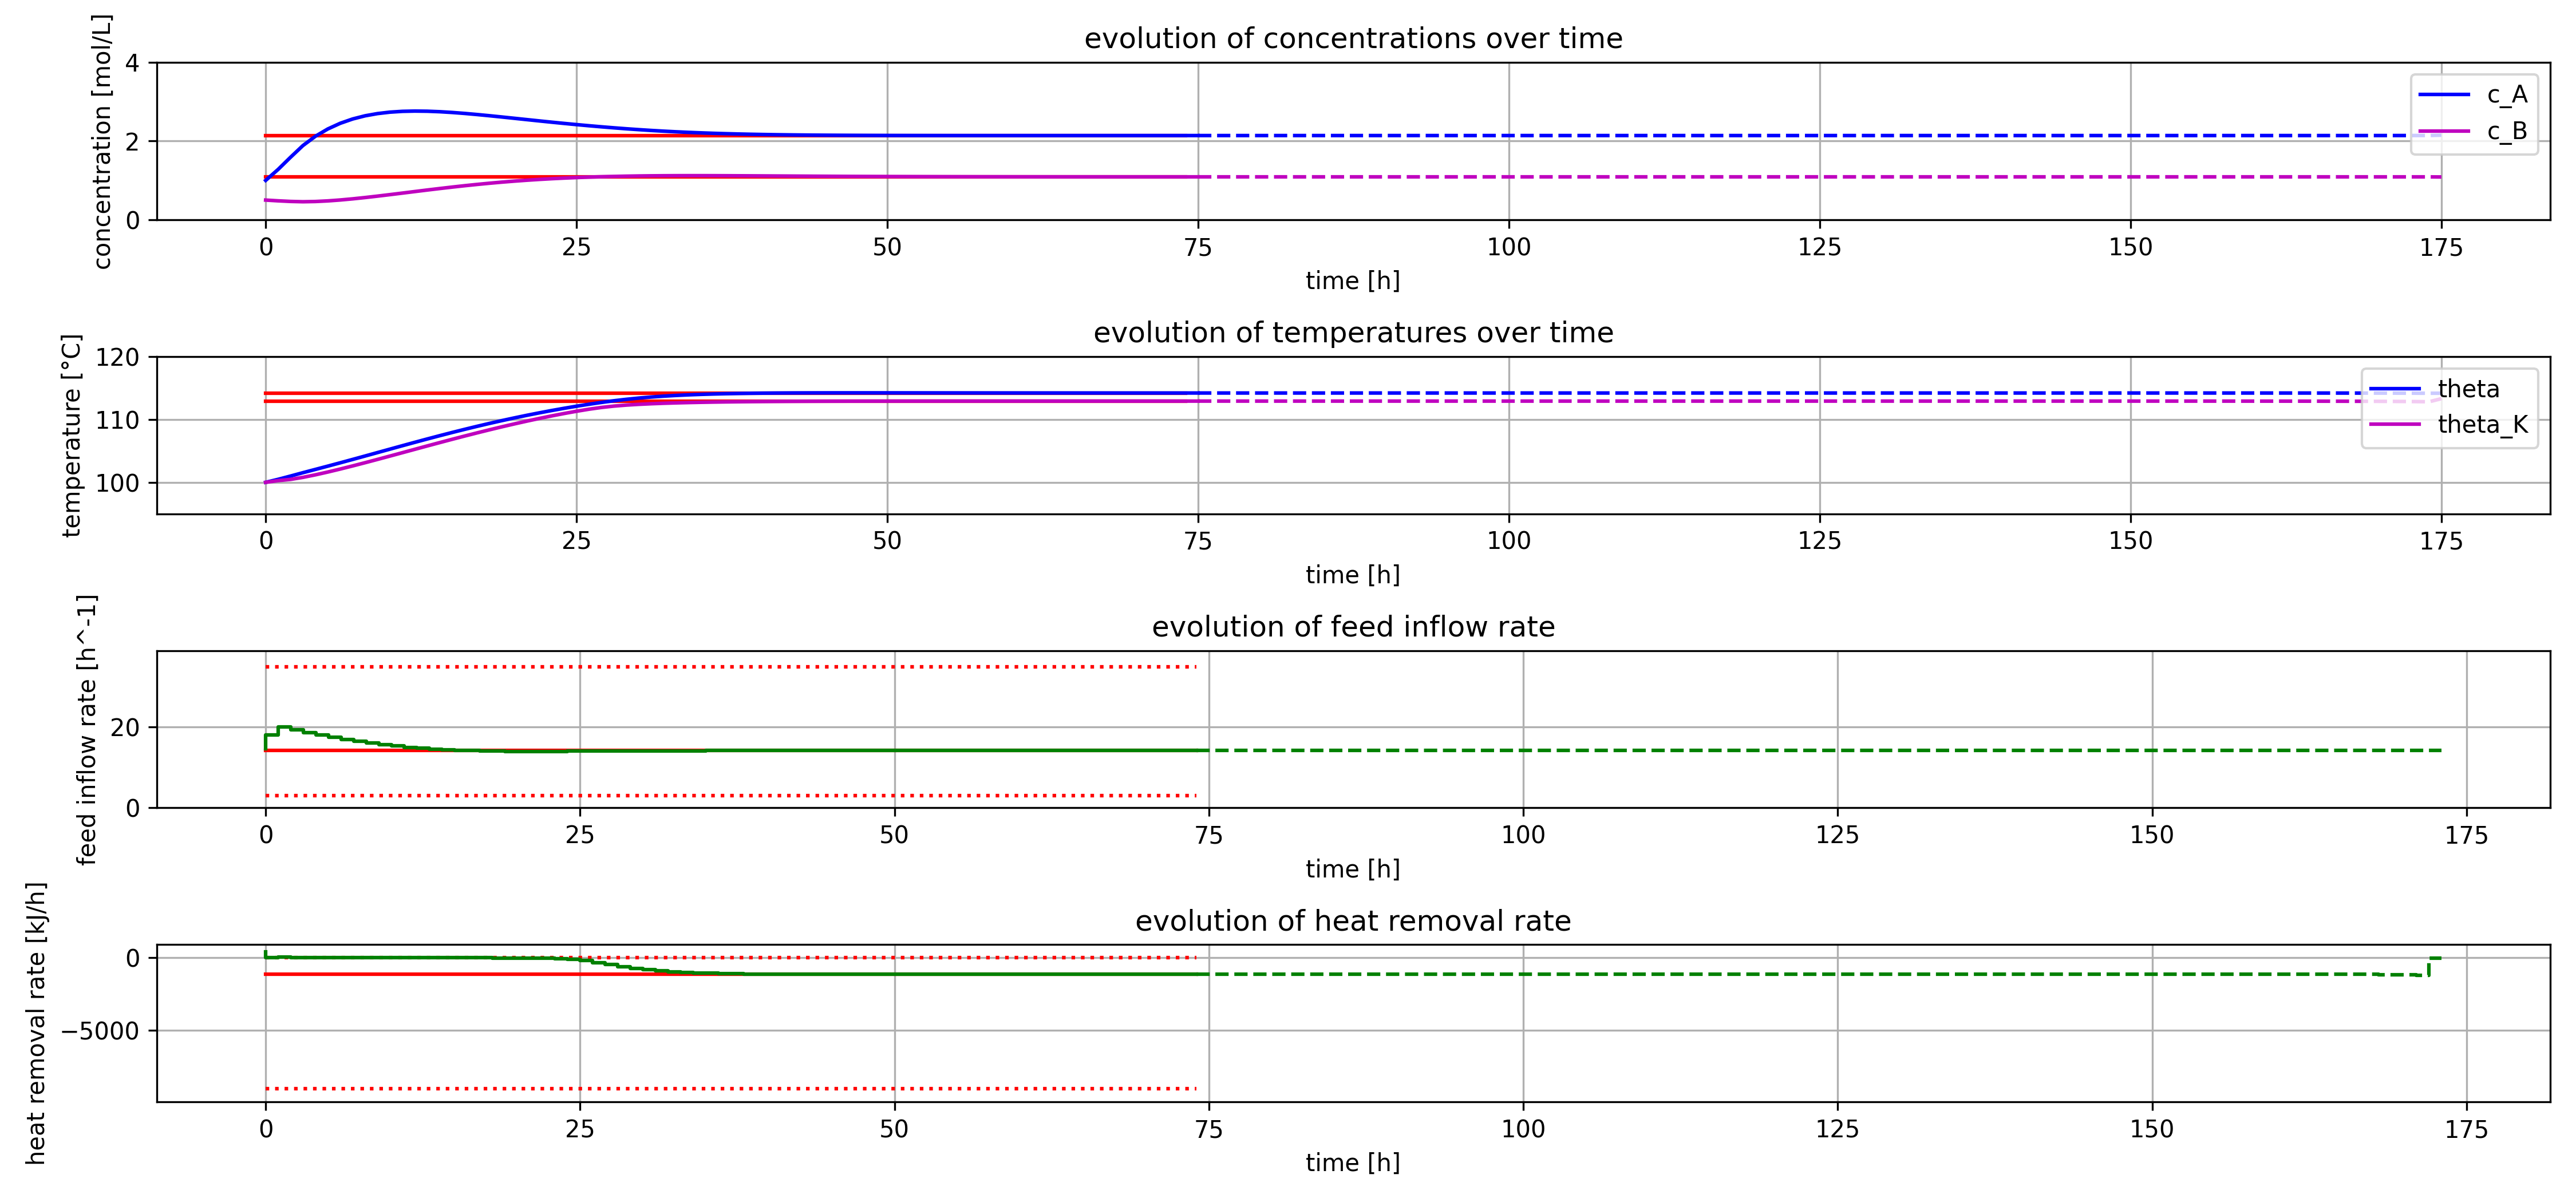
\includegraphics[width=1.0\textwidth]{../cstr_package/rrlb_mpc.png}
        \caption*{Closed-loop trajectories of RRLB MPC}
    \end{figure}
\end{frame}

\begin{frame}
    \frametitle{Numerical experiments - CSTR}
    \begin{figure}[H]
        \centering
        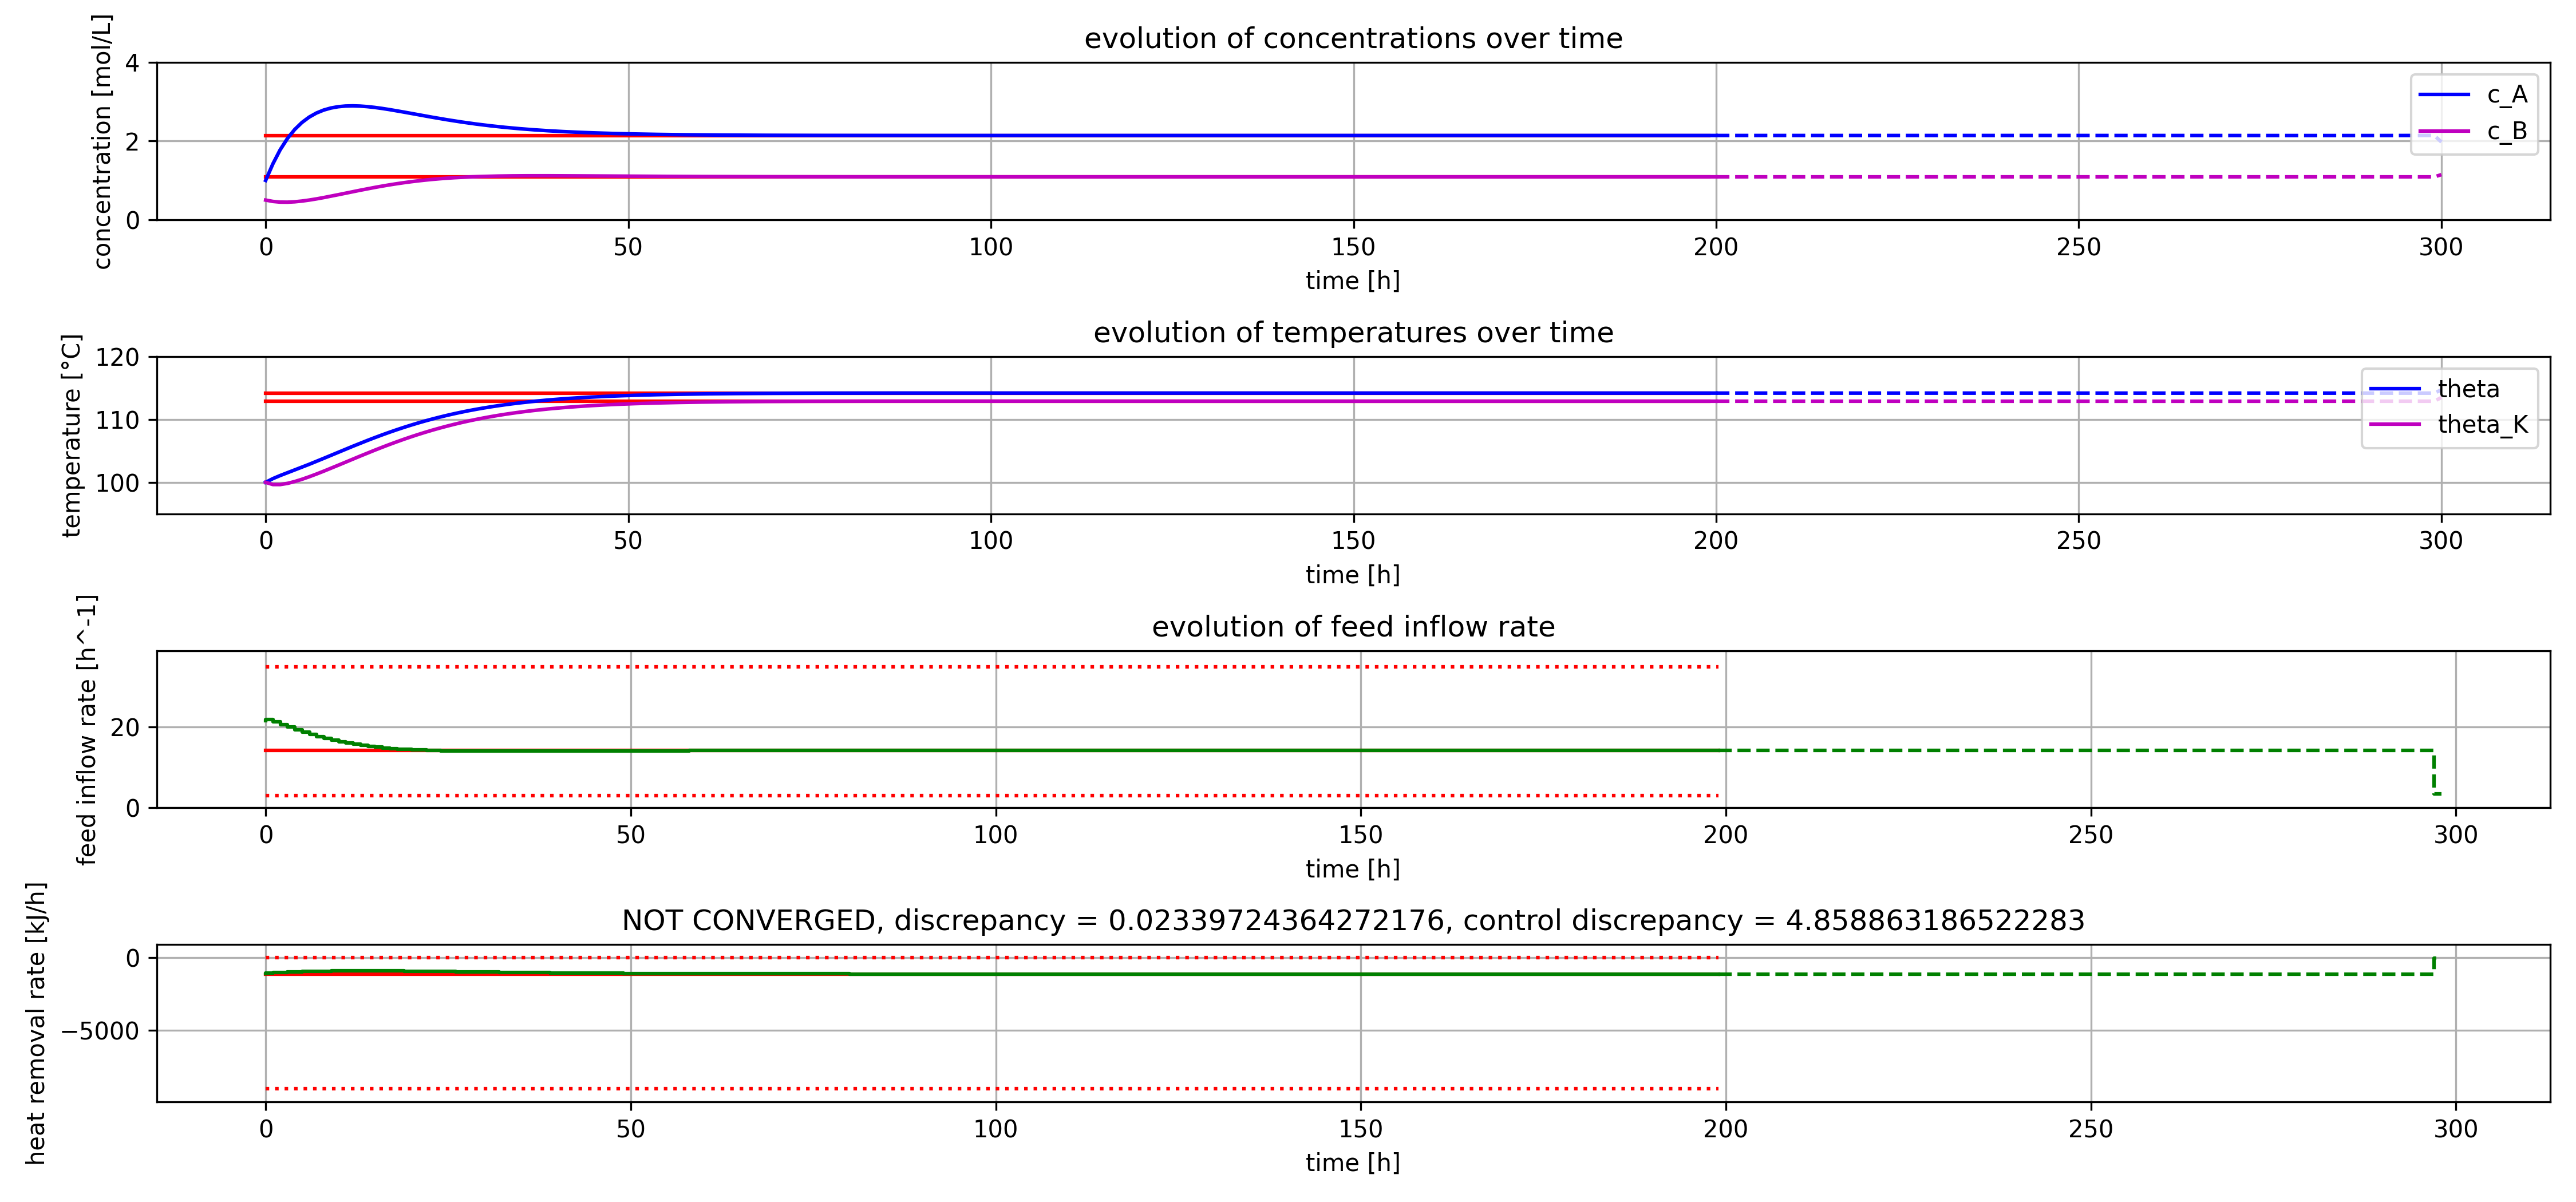
\includegraphics[width=1.0\textwidth]{../cstr_package/mpc.png}
        \caption*{Closed-loop trajectories of MPC}
    \end{figure}
\end{frame}

\begin{frame}
    \frametitle{Numerical experiments - CSTR}    
    % solve times RRLB MPC :
    % mean=25.537693822706068
    % std=2.862889028359942
    % solve times regular MPC :
    % mean=170.89609197668128
    % std=25.23435179106265
    Here are the solve times in ms :\newline
    \begin{minipage}{0.55\textwidth}
        \begin{figure}[H]
            \centering
            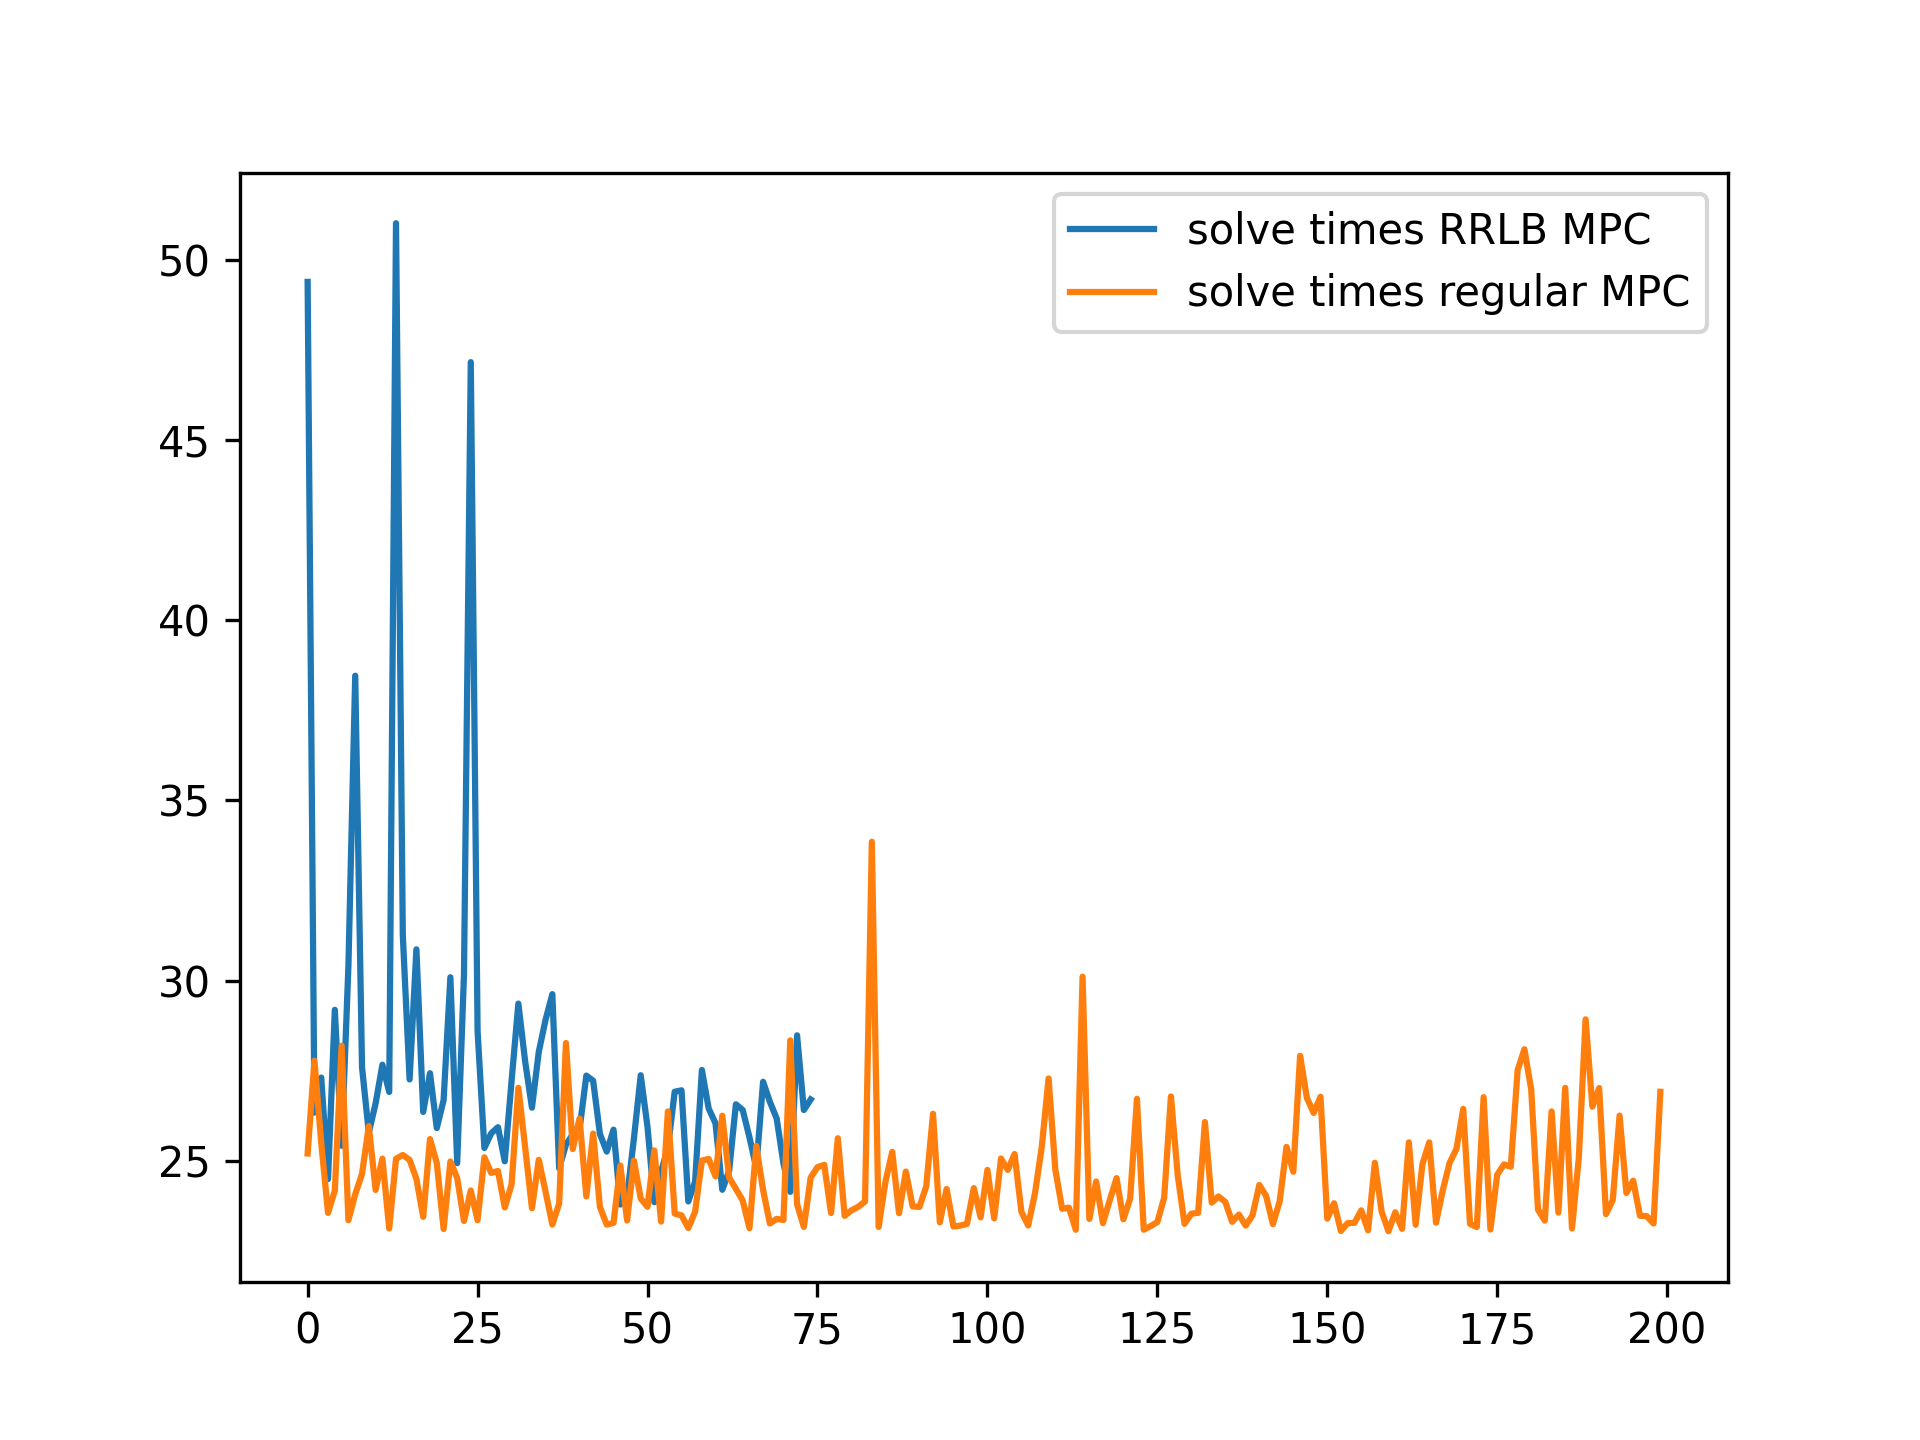
\includegraphics[width=7cm]{../cstr_package/solve_times.png}
            \caption*{Solve times for both schemes}
        \end{figure}
    \end{minipage}
    \begin{minipage}{0.40\textwidth}
        \begin{table}[H]
            \centering
            \begin{tabular}{|c|c|c|}
                \hline
                & mean & stdev\\
                \hline
                RRLB MPC & 25.538 & 2.863 \\
                \hline
                MPC & 170.896 & 25.234 \\
                \hline
              \end{tabular}
        \end{table}
    \end{minipage}
\end{frame}

\end{document}